\documentclass{article}
% Packages
\usepackage{graphicx,subfig,float} % Required for inserting images
\usepackage{amsmath}
\usepackage{datetime}
\usepackage[spanish]{babel}
\usepackage{titling}
\usepackage{geometry}

\geometry{
  a4paper,
  total={170mm,257mm},
  width=150mm,
  height=230mm,
}

\usepackage{tcolorbox}

\graphicspath{{assets/}}

\numberwithin{equation}{section}
\renewcommand{\theequation}{\arabic{section}.\arabic{equation}}

\newenvironment{subs}
  {\adjustwidth{3em}{0pt}}
  {\endadjustwidth}

\providecommand{\abs}[1]{\lvert#1\rvert}


\title{Módulo 2 \\ Conceptos de Arquitectura de Computadoras}
\author{Polanis, Iván Valentín}
\date{}

\begin{document}

\maketitle

\newpage
\tableofcontents
\newpage

\section{Segmentación de instrucciones}

En una arquitectura \textbf{RISC}\footnote{Reduced Instruction Set Computer} la mayoría de las instrucciones son del tipo registro a registro, y un ciclo de instrucción tiene las dos fases siguientes:

\begin{itemize}
  \item \textbf{I}: captación de instrucción
  \item \textbf{E}: ejecución. Realiza una operación de la ALU como entrada y salida.
\end{itemize}

Las operaciones de carga y almacenamiento necesitan tres fases:

\begin{itemize}
  \item \textbf{I}: captación de instrucción
  \item \textbf{E}: ejecución. Calcula una dirección de memoria.
  \item \textbf{D}: memoria. Operación registro a memoria o memoria a registro.
\end{itemize}

Dada la simplicidad y regularidad de un repertorio de instrucciones RISC, el diseño de la organización en tres o cuatro etapas se realiza fácilmente. 

\subsection{Optimización de la segmentación}

Dada la naturaleza sencilla y regular de las instrucciones RISC, los esquemas de segmentación se pueden emplear eficientemente. Hay poca variación en la duración de la ejecución de instrucciones, y el cauce puede adaptarse para reflejar este hecho.

Para compensar las dependencias de datos, se han desarrollado técnicas de reorganización de código. Consideremos primero las instrucciones de salto. El \textit{salto retardado}, que es una forma de incrementar la eficiencia de la segmentación, utiliza un salto que no tiene lugar hasta después de que se ejecute la siguiente instrucción. La posición de la instrucción inmediatamente después de la instrucción de salto se conoce como \textit{espacio de retardo}.

Para saltos condicionales, el procedimiento no puede aplicarse a ciegas. Si la condición comprobada por la bifurcación puede alterarse por la instrucción inmediatamente precedente, el compilador ha de abstenerse de hacer el intercambio en su lugar, debe inserta un NOOP.

Un tipo de táctica similar, llamada \textit{carga retardada}, se puede usar con las instrucciones LOAD. En las instrucciones LOAD, el procesador bloquea el registro destino de la carga. Después el procesador continúa la ejecución del flujo de instrucciones hasta que se alcanza una instrucción que necesite ese registro, deteniéndose hasta que la carga finalice. Si el compilador puede reorganizar las instrucciones de manera que se pueda hacer un trabajo útil mientras la carga está en el cauce, la eficiencia aumenta.


\section{Soluciones a Atascos}

\subsection{Soluciones a riesgos estructurales}

La solución es simple, se debe replicar, segmentar o realizar turnos para el acceso a las unidades funcionales en conflicto.

\begin{itemize}
  \item Duplicación de recursos de hardware.
  \subitem{Sumadores o restadores además de la ALU.}
  \item Separación en memorias de instrucciones y datos.
  \item Turnar el acceso al banco de registro.
  \subitem{Escrituras en la primera mitad del ciclo de reloj.}
  \subitem{Lecturas en la segunda mitad del ciclo de reloj.}
\end{itemize}

\subsection{Soluciones a riesgos de datos}

Para riesgos \textbf{RAW} se debe determinar cómo y cuando aparecen esos riesgos. Para ello será necesario una unidad de detección de riesgos y/o un compilador más complejo.

Para este tipo de riesgo tenemos dos soluciones:

\begin{itemize}
  \item \textbf{Hardware}
  \subitem{Adelantamiento de operandos (Forwarding).}
  \item \textbf{Software}
  \subitem{Instrucciones NOP o reordenamiento de de codigo.}
\end{itemize}

\subsubsection{Adelantamiento de operandos (Forwarding)}

Esta técnica consiste en pasar directamente el resultado obtenido con una instrucción a las instrucciones que lo necesitan como operando. Si el dato necesario está disponible a la salida de la ALU ($X_i$) se lleva a la entrada de la etapa correspondiente ($X_{i+1}$) sin esperar a la escriturar ($M_i$ o $W_i$).

\begin{figure}[H]
  \centering
  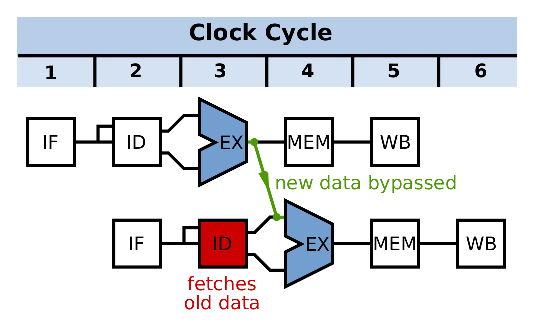
\includegraphics[width=0.7\textwidth]{Forwarding}
  \caption{Adelantamiento de operandos.} 
\end{figure}

\subsubsection{Instrucciones NOP o reordenamiento de código}

Evita los riesgos reordenando las instrucciones del código sin afectar el código. El compilador es el encargado de realizar esta tarea.

Aquí se introducen las instrucciones NOP, que son utilizadas para generar un retardo. Estas instrucciones no realizan ninguna operación, pero consumen un ciclo de reloj. Ademas, se reordenan instrucciones para evitar riesgos RAW.\@

\subsection{Soluciones a riesgos de control}

En los riesgos de control se introduce la penalización por salto. Cuando el salto es incondicional, la dirección de destino se debe determinar lo más pronto posible, dentro del cauce, para reducir la penalización. Cuando el salto es condicional, la penalización se debe a que el procesador no sabe si se debe tomar o no el salto hasta que se evalúe la condición.

Se utiliza una modificación sencilla de la ruta de datos para reducir la cantidad de paradas a un solo ciclo:

\begin{itemize}
  \item \textbf{Adelantar la resolución de los saltos a la etapa D}
  \begin{itemize}
    \item En ella se decodifica y se sabe que es un salto.
    \item Se puede evaluar la condición de salto.
    \item Se puede calcular la dirección de destino.
  \end{itemize}
\end{itemize}

\subsubsection{Técnicas de predicción de salto (Hardware)}

Para este tipo de técnicas tenemos dos posibilidades:

\begin{itemize}
  \item \textbf{Predicción estática}
  \subitem{Se asume que el salto se toma o no se toma.}
  \item \textbf{Predicción dinámica}
  \subitem{Se utiliza un predictor de saltos.}
\end{itemize}

\subsubsection*{Predicción estática}

\begin{itemize}
  \item \textbf{Predicción de salto tomado}
  \subitem{Se asume que el salto se toma.}
  \subitem{Se adelanta la búsqueda de la dirección de destino.}
  \item \textbf{Predicción de salto no tomado}
  \subitem{Se asume que el salto no se toma.}
  \subitem{Se continúa con la ejecución secuencial.}
\end{itemize}

\subsubsection*{Predicción dinámica}

\begin{itemize}
  \item \textbf{Conmutador saltar/no saltar}
  \begin{itemize}
    \item Basado en la historia de las instrucciones.
    \item Es eficaz para los bucles.
  \end{itemize}
  \item \textbf{Tabla de historia de saltos (BTB)}
  \begin{itemize}
    \item Pequeña cache asociada a la etapa de búsqueda (F).
    \item Contiene tres campos.
    \subitem{Dirección de una instrucción de bifurcación.}
    \subitem{Información de la instrucción destino.}
    \subitem{N bits de estado (histórico).}
  \end{itemize}
\end{itemize}

\subsubsection*{Otras soluciones}

Una técnica que se utiliza es la \textbf{predicción según el código de operación}, ya que existen instrucciones con más probabilidades de saltar. La tasa de acierto es del 75\%.

Los \textbf{Flujos múltiples} utilizan varios cauces (uno por cada opción de salto). Precaptan cada salto en diferentes cauces. Las desventajas son que provoca retardos en el acceso al bus y a los registros. Si hay múltiples saltos, se necesita un mayor número de cauces.

La \textbf{Precaptación del destino de salto} consiste en precaptar la instrucción destino del salto, además de las instrucciones siguientes a la bifurcación. La instrucción se guarda hasta que se ejecute la instrucción de bifurcación.

En el \textbf{Buffer de bucles} se utiliza una memoria muy rápida gestionada por la etapa de captación de instrucción del cauce. Comprueba el buffer antes de hacer la captación de memoria. Esta técnica es muy eficaz para pequeños bucles y saltos.

\subsubsection{Instrucciones de salto retardado (Software)}

La idea es realizar trabajo útil mientras el salto se resuelve.

\begin{itemize}
  \item Hueco o ranura de retardo de salto es el período de penalización o parada luego de una instrucción de salto.
  \item El compilador trata de situar instrucciones útiles (que no dependan del salto) en los huecos de retardo. Si no es posible, se utilizan instrucciones NOP.\@
  \item Las instrucciones en los huecos de retardo de salto se captan siempre.
  \item Requiere reordenamiento de código.
\end{itemize}
\section{Computadoras de repertorio reducido de instrucciones}

Algunos de los principales avances desde el nacimiento del computador son:

\begin{itemize}
  \item \textbf{El concepto de familia:} introducido por IBM en su System/360 em 1964. El concepto de familia separa la arquitectura de una máquina de su implementación. Se ofrece un conjunto de computadores, con distintas características en cuanto a precio/prestaciones, que presentan al usuario la misma arquitectura.
  \item \textbf{Unidad de control micro programada:} propuesta por Wilkes en 1951, e introducida por iBM en la línea S/360 en 1964. La micro programación facilita la tarea de diseñar e implementar la unidad de control y da soporte al concepto de familia.
  \item \textbf{Memoria caché:} introducida en 1968 por IBM.\@ La introducción de este elemento en la jerarquía de memoria mejoró las prestaciones de manera espectacular.
  \item \textbf{Segmentación de cauce:} una manera de introducir procesamiento simultaneo en la naturaleza esencialmente secuencial de un por instrucciones máquina.
\end{itemize}

La arquitectura RISC se aparta de manera drástica de la tendencia histórica en la arquitectura del procesador. Un análisis de la arquitectura RISC involucra la mayoría de los asuntos importantes de organización y arquitectura de computadores.

Los sistemas RISC están caracterizados por:

\begin{itemize}
  \item Un gran número de registros de uso general, o el uso de tecnología de compiladores para optimizar la utilización de los registros.
  \item Un repertorio de instrucciones limitado y sencillo.
  \item Un énfasis en la optimización de la segmentación de instrucciones.
\end{itemize}

\subsection{Características de la ejecución de instrucciones}

Los repertorios complejos de instrucciones están pensados para:

\begin{itemize}
  \item Facilitar el trabajo del escritor de compiladores.
  \item Mejorar la eficiencia de la ejecución, ya que las secuencias complejas de operaciones pueden implementarse en micro código.
  \item Dar soporte a HLL\footnote{High Level Language} aun más complejos y sofisticados.
\end{itemize}

Para comprender la línea de razonamiento de los partidarios de los RISC, comenzamos con una breve revisión de las características de la ejecución de instrucciones. Los aspectos cuyo cálculo tiene interés son los siguientes:

\begin{itemize}
  \item \textbf{Operaciones realizadas:} determinan las funciones que lleva a cabo el procesador y su interacción con la memoria.
  \item \textbf{Operandos usados:} los tipos de operandos y su frecuencia de uso determinan la organización de memoria para almacenarlos y los modos de direccionamiento para acceder a ellos.
  \item \textbf{Secuenciamiento de la ejecución:} determina la organización del control y del cauce segmentado.
\end{itemize}

\subsubsection*{Operaciones}

Existe una gran concordancia en los resultados de esta mezcla de lenguajes y aplicaciones. Las sentencias de asignación predominan, lo cual indica que el sencillo movimiento de datos tiene mucha importancia. También predominan las sentencias condicionales (IF, LOOP). Estas sentencias se implementen en el lenguaje máquina con alguna instrucción del tipo comparar y saltar. Esto indica que el mecanismo incluido en el repertorio de instrucciones para el control del secuenciamiento es importante.

Estos resultados son instructivos para el diseñador del repertorio de instrucciones máquina, diciéndole qué tipo de sentencias tiene lugar más a menudo y por consiguiente deben ser implementadas de una forma óptima.

\subsubsection*{Operandos}

EL estudio de Patterson ya referenciado también consideró la frecuencia dinámica de aparición de distintas clases de variables. Los resultados, coherentes para programas en Pascal y en C, muestran que la mayoría de las referencias se hacen a variables escalares simples. Además, más del ochenta por ciento de los datos  eran variables locales. Asimismo, las referencias a matrices/estructuras requieren una referencia previa a su índice o puntero, que nuevamente suele ser un dato escalar local. Por consiguiente, hay un predominio de referencias a operandos escalares, y estos están muy localizados.

Estos estudios reflejan la importancia de una arquitectura que se preste a un rápido acceso a operandos, dado que es una operación que se realiza con mucha frecuencia. El estudio de Patterson indica que un candidato fundamental a optimizar es el mecanismo de almacenamiento y acceso a variables escalares.

\subsubsection*{Llamadas a procedimientos}

Las llamadas y retornos de procedimientos constituyen un aspecto importante de los programas en HLL.\@ Los estudios indican que son las operaciones que consumen más tiempo en programas en HLL compilados.

Esto depende del número de parámetros tratados y del nivel de anidamiento. La mayoría de los programas no tienen una larga secuencia de llamadas seguida por la correspondiente secuencia de retornos. Además la mayoría de las variables suelen ser locales y las referencias a operandos están muy localizadas.

Partiendo del trabajo de varios investigadores, surgen tres elementos que, por lo general, caracterizan las arquitecturas RISC:\@

\begin{itemize}
  \item \textbf{Utilización de un amplio banco de registros}
  \item \textbf{Cuidadosa atención al diseño de los cauces de instrucciones.}
  \item \textbf{Uso de un repertorio simplificado de instrucciones}
\end{itemize}

\subsection{Utilización de un amplio banco de registros}

Se necesita una estrategia que permita que los operandos a los que se acceda con mayor frecuencia se encuentren en registros y se minimicen las operaciones registro-memoria.

Son posibles dos aproximaciones básicas, una basada en software y la otra en hardware.

La aproximación por software consiste en confiar al compilador la maximización del uso de los registros. El compilador intentará asignar registros a las variables que se usen más en un periodo dado. Esta solución requiere el uso de sofisticados algoritmos de análisis de programas.

La aproximación por hardware consiste sencillamente en usar más registros de manera que puedan mantenerse en ellos más variables durante períodos de tiempo más largos.

\subsubsection*{Ventanas de registros}

A primera vista, el uso de un conjunto amplio de registros debería reducir la necesidad de acceder a memoria. La labor del diseño es organizar los registros de tal modo que se alcance esa meta.

Una llamada a un procedimiento hace que el procesador conmute automáticamente a una ventana de registros distinta de tamaño fijo, en lugar de salvaguardar los registros en memoria. Las ventanas de procedimientos adyacentes están parcialmente solapadas para permitir el paso de parámetros.

La ventana se divide en tres áreas de tamaño fijo. Los registros de parámetros contienen parámetros pasados al procedimiento actual desde el procedimiento que lo llamó, y los resultados a devolver a este. Los registros locales se usan para variables locales, según la asignación que realice el compilador. Los registros temporales se usan para intercambiar parámetros y resultados con el siguiente nivel más bajo (el procedimiento llamado por el procedimiento en curso). Los registros temporales de un nivel son físicamente los mismos que los registros de parámetros del nivel más bajo adyacente. Este solapamiento posibilita que los parámetros se pasen sin que exista una transferencia de datos real.

Para manejar cualquier patrón posible de llamadas y retornos, el número de ventanas de registros tendría que ser ilimitado. En lugar de eso, las ventanas de registros se pueden usar para contener unas pocas, las más recientes, activaciones de procedimientos. Las activaciones más antiguas han de salvaguardarse en memoria y restaurarse más tarde cuando la profundidad de anidamiento disminuya.

\begin{figure}[H]
  \centering
  \includegraphics[width=0.5\textwidth]{Buffer.png}
  \caption{Organización de las ventanas solapadas con un buffer circular.}
\end{figure}

\subsubsection*{Variables Globales}

Para tratar variables globales se sugieren dos opciones.

La primera es que el compilador asigne posiciones de memoria a las variables declaradas como globales en un HLL, y que todas las instrucciones máquina que referencien esas variables declaradas como globales en un HLL, y que todas las instrucciones máquina que referencien esas variables usen operandos referenciados en memoria.

Una alternativa es incorporar al procesador un conjunto de registros globales. Estos registros serían fijos en cuanto a su número y accesibles por todos los procedimientos. Se puede usar un esquema de numeración unificado para simplificar el formato de instrucción. Esto conlleva un hardware añadido, que se encarga de adaptar la división en el direccionamiento de los registros.

\subsubsection*{Un amplio banco de registros frente a una caché}

\begin{table}
\centering
\begin{tblr}{
  width = \linewidth,
  colspec = {Q[488]Q[452]},
  row{1} = {c},
  hlines,
  vlines,
}
\textbf{Banco de registros amplio}                   & \textbf{Caché}                                   \\
Todos los datos escalares locales                    & Datos escalares locales recientemente usados     \\
Variables individuales                               & Bloques de memoria                               \\
Variables globales asignadas por el compilador       & Variables recientemente                          \\
Salvaguarda basadas en la profundidad de anidamiento & Salvaguarda basadas en el algoritmo de reemplazo \\
Direccionamiento a registros                         & Direccionamiento a memoria                       
\end{tblr}
\end{table}

\subsection{Optimización de registros basada en el compilador}

Supongamos que ahora disponemos de una máquina RISC que contiene unicamente un pequeño número de registros. En ese caso, el uso optimizado de registros es responsabilidad del compilador. Los programas escritos en HLL no tienen referencias explicitas a los registros. El objetivo del compilador es mantener en registros en lugar de en memoria los operandos necesarios para tantos cálculos como sea posible, y minimizar las operaciones de carga y almacenamiento.

Por lo general se sigue el siguiente enfoque. Cada cantidad del programa candidata para residir en un registro se asigna a un registro simbólico o virtual. El compilador entonces asigna el número ilimitado de registros simbólicos a un número fijo de registros reales. Los registros simbólicos cuya utilización no se solape pueden compartir el mismo registro real. Si en una parte concreta del programa hay más cantidades a tratar que registros reales, algunas de las cantidades se asignan a posiciones de memoria.

\subsection{Arquitectura de repertorio reducido de instrucciones}

\subsubsection*{¿Por qué CISC?}

La primera de las razones es, la simplificación de los compiladores. La labor del escritor de compiladores es generar una secuencia de instrucciones máquina para cada sentencia HLL.\@ Se existen instrucciones máquina que se parezcan a sentencias del HLL, la tarea se simplifica.

La otra razón importante mencionada es la esperanza de que un CISC produzca programas más pequeños y rápido. Los programas más pequeños tienen dos ventajas. Como el programa ocupa menos memoria, hay un ahorro de este recurso, pero como la memoria hoy en día es tan barata, este aspecto no es primordial. Tiene mayor importancia el hecho de que programas más pequeños mejoren las prestaciones porque tienen menos instrucciones, lo que significa que hay que captar menos bytes de instrucciones. El segundo es que en un entorno paginado los programas más pequeños ocupan menos páginas, reduciendo los fallos de página. Sin embargo, el número de bits de memoria que ocupa, no tiene por qué ser más pequeño al tener menos instrucciones.

El segundo factor que motivaba repertorios de instrucciones cada vez más complejos era que la ejecución de instrucciones fuera más rápida. Parece tener sentido el que una operación compleja de un HLL se ejecute más rápido como una única instrucción máquina que como una sucesión de instrucciones más primitivas. Sin embargo, debido a la propensión a usar las instrucciones más sencillas, esto puede no ser así. La unidad de control completa debe hacerse más compleja, y/o la memoria de control del micro programa ha de hacerse más grande, para acomodar un repertorio de instrucciones más rico.

\subsubsection*{Características de RISC}

\begin{itemize}
  \item Una instrucción por ciclo.
  \item Operaciones registro a registro.
  \item Modos de direccionamiento sencillos.
  \item Formatos de instrucción sencillos.
\end{itemize}

Un \textit{ciclo máquina} se define como el tiempo que se tarda en captar dos operandos desde dos registros, realizar una operación de la ALU y almacenar el resultado en un registro. Así, las instrucciones máquina de un RISC no deberían ser más complicadas que las micro instrucciones de las máquinas CISC, y deberían comportarse más o menos igual de rápido.

Una segunda característica es que la mayoría de las operaciones deben ser del tipo \textbf{registro a registro} con la excepción de sencillas operaciones LOAD y STORE para acceder a memoria. 

Casi todas las instrucciones RISC usan direccionamiento sencillo a registro. Se pueden incluir varios modos adicionales, como el desplazamiento y el relativo al contador de programa. 

Por último, solo se usa un formato o unos pocos. La longitud de las instrucciones es fija y alineada en los limites de una palabra. Las posiciones de los campos, especialmente la del código de operación, son fijas.

\appendix

\end{document}
